\section{Overall Description}\label{intro}
\subsection{Product perspective}
\subsubsection{Scenarios}
\begin{enumerate}[label=\textbf{\Alph*}.]
    \item  \textbf{Educator Registration} \\
    Marco, an educator at the University of Naples, recently discovered the CKB platform
platform thanks to a colleague. Interested in its potential to improve students' software development skills, Marco decided to
software development skills of students, Marco decided to register as an educator. Visiting the home page of
CKB home page, he selected the "Register" option and entered his email address, chose a password
and provided his first and last name. After entering this information, Marco was asked to
verify his email by clicking on a link sent to him to ensure the security of his account. Once
Once this verification was completed, he proceeded with the registration by selecting the option "Sign up
as educator" option. With the registration successfully completed, Marco was redirected to his
personal dashboard within CKB, where he had access to an overview of the functionalities
for educators, including the possibility to create new tournaments and battles.
\item  \textbf{Student Registration} \\
Andrea, a student at the University of Bologna, discovered the CKB application thanks to the advice
of his professor. Fascinated by the opportunity to hone his software development skills
through code kata challenges, Andrea decided to subscribe to the platform. Once on the home
page of CKB, he selected the "Register" option and provided his email address, creating a
password. She also entered her first and last name, selecting the "Register as a student" option
to complete the registration. However, before finalising the process, the system prompted
Andrea to verify his email address by clicking on a link sent to him, to ensure the authenticity of his account.
of her account. During this step, Andrea received an error message: the
address was already present in the CKB system. He promptly corrected the email address, using a valid account.
a valid account. Once he had successfully verified his email and completed the
registration process, Andrea was redirected to his personal dashboard on CKB. Here, he was able to
explore the various features available to students, such as active tournaments, upcoming competitions
upcoming competitions and information about her progress on the platform.
    \item \textbf{Tournament Creation} \\ 
    Daniele, a professor of computer science at the Politecnico di Milano, would like to create a tournament on the
CKB platform to allow his students to develop and improve their
programming skills through participation in code kata battles.
Daniele accesses the platform using his login credentials as a professor and navigates
to the section dedicated to the creation of tournaments on the CKB platform.
He then starts the process of creating a new tournament by selecting the appro- priate option from the main dashboard.
selected from the main dashboard. The system prompts Daniel to enter information about the tournament,
such as the name, a deadline for students to register for the tournament and the list
of colleagues who can create battles within that tournament.
The teacher completes the form and, after entering the required information, confirms the creation
of the tournament. The system verifies the validity of the information provided and, if the name of the tournament
If the name of the tournament already exists, the system sends the following warning: "The name of the tournament already exists". Otherwise, in
In the event of positive verification, the system registers the new tournament within the system. All students
registered on the platform receive notifications about the creation of the new tournament.
\item \textbf{Battle Creation} \\ 
John, a professor with battle creation privileges within the 'Algorithms and
data structures' on the CKB platform, decides to create a new battle. To this end, after
logging in, he navigates to the battle creation section and starts the process of creating a new battle.
of creating a new battle. The system prompts Daniel to enter essential information about the battle, including an
battle, including a short textual description, the software project with the scripts for
automation of the build, the minimum and maximum number of students per group, the expiry date
for registration and delivery of the project. In addition, Daniele sets additional information
that will affect the scoring, such as security, maintenance and affid-
ability. Finally, the system integrates the new battle into the platform. Students registered for the tournament
relevant tournament receive notifications about the next battle.
\newpage
\item \textbf{Tournament registration} \\
Sarah, a computer engineering student, finds herself eager for a new challenge to raise her programming skills. She then decides to log onto the CKB platform. After logging in, she explores the section on available tournaments and spots one in particular - "Python Challenge". Sarah clicks on the tournament and reads its description and notices that the deadline for registration has not expired. Without hesitation, she decides to participate in the Python Challenge. By clicking on 'Join the tournament' Sarah receives a confirmation message and is officially part of the tournament. She can now view all scheduled battles within the tournament and will also be notified when future battles are created.

\item \textbf{Battle registration} \\
Leonardo, a student enrolled in the "Super Tournament" on CKB, receives a notification that catches his attention: "Call to Battle - Python Coding Challenge". Keen to put his programming skills to the test, Leonardo, after logging in, enters the section dedicated to the battle, carefully reads the details provided and decides to sign up for the battle by clicking on "Join the battle". Subsequently, the platform allows Leonardo to choose whether to participate individually or invite other colleagues to form a team for the battle, respecting the minimum and maximum number of participants allowed. The platform only allows Leonardo to invite students who do not already have a team for the respective battle. After the registration phase has expired, the CKB platform automatically generates a dedicated repository for the 'Python Coding Challenge' project. Subsequently, the direct link to the repository is delivered to team members and made available in the "Your Battles" section of the application.
\item  \textbf{Face the battle} \\
The 'CodeCrafters' team, consisting of enthusiastic students eager to immerse themselves in the battle, receives by e-mail the link to the repository on GitHub dedicated to the 'Advanced Algorithms' challenge on CKB. With a simple click, they proceed to fork that repository, containing the kata code, thus creating their own virtual workspace. To ensure continuous and accurate evaluation of their work, CodeCrafters configure GitHub Actions, which ensures timely communication with the platform.
Immersed in the exciting challenge of 'Advanced Algorithms', CodeCrafters start the development process by adopting the test-first approach. Creatively, they create the first implementations, test them and commit them to the main repository, thus tracking every step of their iterative journey. Each push before the battle deadline activates the platform, which automatically evaluates the functional aspects and timeliness of the CodeCrafters' work. Subsequently, the platform calculates and updates their battle score, offering real-time feedback on the quality of their valuable contribution.
\item \textbf{Battle elimination} \\
Luca, an educator in computer science at  'Politecnico di Milano', decides to delete a battle in a tournament for which he has permissions, due to the low number of registered teams. After logging into the system, he navigates to the battles section of a specific tournament and selects the battle he wishes to remove. If the entry date for that battle has not yet expired or the battle has ended, he is given the option to click on "Remove Battle". By proceeding with 'Confirm' on a confirmation message, Luke finalises his decision. Once the action has been confirmed, the system automatically sends an e-mail to all students who are part of the teams registered for that battle, informing them that the battle has been eliminated. This process ensures that students are promptly informed of any changes to their activities in the tournament by e-mail.
\item \textbf{Ranking display} \\
Matthew, while participating in a battle on CKB, can monitor his team's position in real time through a dynamic ranking by logging into the tournament and battle section of interest. At the end of the battle, he is faced with a consolidation phase, during which the educator can decide whether to assign a personal score to the project or rely solely on the automatic scoring. At the conclusion of this phase, Matthew can consult the final ranking by going to the section dedicated to the battle that has just ended, thus obtaining a complete overview of his team's performance.

The score obtained in this specific battle is added to those accumulated in previous battles, contributing to his overall score in the tournament. Matthew and all users have the possibility to explore the ranking in the section dedicated to the tournament itself, accessible to all interested users.

Finally, once the educator definitively closes the tournament, Matteo and the other CKB members can consult the final ranking of the tournament in the section relating to that tournament.

\item \textbf{Evaluates project} \\
Once the submission phase of a battle of the "Advanced Algorithms" tournament on CKB has expired, Professor Bianchi, the creator of the challenge, prepares to perform a manual evaluation of the projects submitted by the participating teams.He logs onto the platform, selects the tournament and the battle that has just ended. Within the interface, he finds a complete list of student projects if manual evaluation was added during the creation of the battle.
Start by carefully examining the source code produced by each team, analysing the aspects that cannot be fully evaluated automatically.
During this phase, Professor Bianchi assigns a personal score to each team based on his experience and in-depth knowledge, in particular rewarding the creativity, ingenuity and strategic approach of the participating teams. Once the evaluation is complete, the final score for each team is determined by averaging the score assigned manually by Professor Bianchi and the score generated automatically by the platform.
\item \textbf{Tournament Closure}\\
Luisa, a lecturer in computer science at the University of Turin, has successfully run the "Logic Masters" tournament on the CKB platform.After the last battle, she decides to close the tournament.Luisa logs in to CKB with her credentials and navigates to the "Logic Masters" tournament section.In the tournament dashboard, she finds the option "Close the Tournament".	After clicking on this option, a warning message appears: "Are you sure you want to close the tournament?".
Luisa must choose between "Confirm" to proceed with the closing or "Cancel" to abort the operation. Upon confirmation of closure, the system closes the tournament if there are still no active battles.
\item \textbf{Tournament Elimination}\\
Luigi, a professor registered on the CKB platform, decides to remove a tournament he had previously created. After completing all the planned battles within the tournament, Luigi proceeds with the removal. He navigates to the 'Tournament' section of the platform and accesses the page of the specific tournament. There, he finds and presses the 'Delete Tournament' button. A confirmation message appears, asking if Luigi is sure he wants to proceed with the deletion. Upon answering 'Yes', the system starts the process of deleting the tournament.
Before permanently removing the tournament, the platform performs a check to ensure that there are no battles still in progress. If it finds an active battle, the system interrupts the elimination process and displays an 'elimination error' message indicating that the tournament cannot be eliminated at that time due to the presence of ongoing activity. 
\end{enumerate}
\subsubsection{User interface}
The system needs to interact with users via devices that require an internet connection. To access the system, all users must connect through a web interface hosted on an existing domain, such as www.codekatabattle.com.
\subsubsection{Software interface}
The system will use some  external interfaces in order to accomplish its functionalities.
\begin{enumerate}
    \item The system is required to retrieve data from  database, necessitating the implementation of  interfaces to ensure accurate data retrieval.
    \item The system interacts with external APIs to offer email notification services.
    \item The system interacts with GitHub to create and manage repositories for code kata exercises. It sets up automated workflows using GitHub Actions to track code commits, trigger updates, and calculate battle scores.
\end{enumerate}
\subsubsection{Interfaccia Hardware}

CKB è accessibile da una varietà di dispositivi hardware, garantendo un'esperienza utente ottimale su diverse piattaforme. Di seguito sono elencati i principali dispositivi hardware supportati:

\begin{itemize}
    \item Computer Desktop e Laptop

    \item Smartphone e Tablet 

\end{itemize}






\subsection{Domain class diagram}
In the figure is represented the domain class diagram related to CKB. This diagram is used  to represent the key concept of our system and the interaction between them.
The main elements of the diagram are:
\begin{itemize}
    \item The 'User' class is responsible for representing users within the system. It is divided into two specialized subclasses: 'Educator' and 'Student.' This division allows for the more effective management of specific functionalities and behaviors for each type of user. Educators have the ability to create tournaments and battles within the system. Students have the opportunity to enroll in tournaments created by educators and participate in battles.
    \item The 'Tournament' class represents tournaments within the system. It possesses a crucial attribute known as 'Educator Permissions.' This attribute serves the purpose of indicating which educators have the authorization,given by the tournament's creator, to create battles within that specific tournament.
    \item  The 'Automated Evaluation' class represents an evaluation process that is automated and consistently carried out. It encompasses predefined parameters and criteria to assess specific elements automatically. Furthermore, 'Manual Evaluation' is a specialized form of evaluation within the system, and it extends from the 'Automated Evaluation' class. It shares the same predefined parameters and criteria as automated evaluation, but with the added capability of manual assessment by educators. Unlike automated evaluations, manual evaluations are not performed automatically but are initiated at the discretion of educators. Educators have the flexibility to decide whether to conduct a manual evaluation or not, enhancing the evaluation process when educator intervention is desired
\end{itemize}

\begin{figure}[h] % [h] indica che LaTeX dovrebbe cercare di posizionare l'immagine qui, ma potresti utilizzare anche altre opzioni come [htbp]
  \centering % Centra l'immagine orizzontalmente
  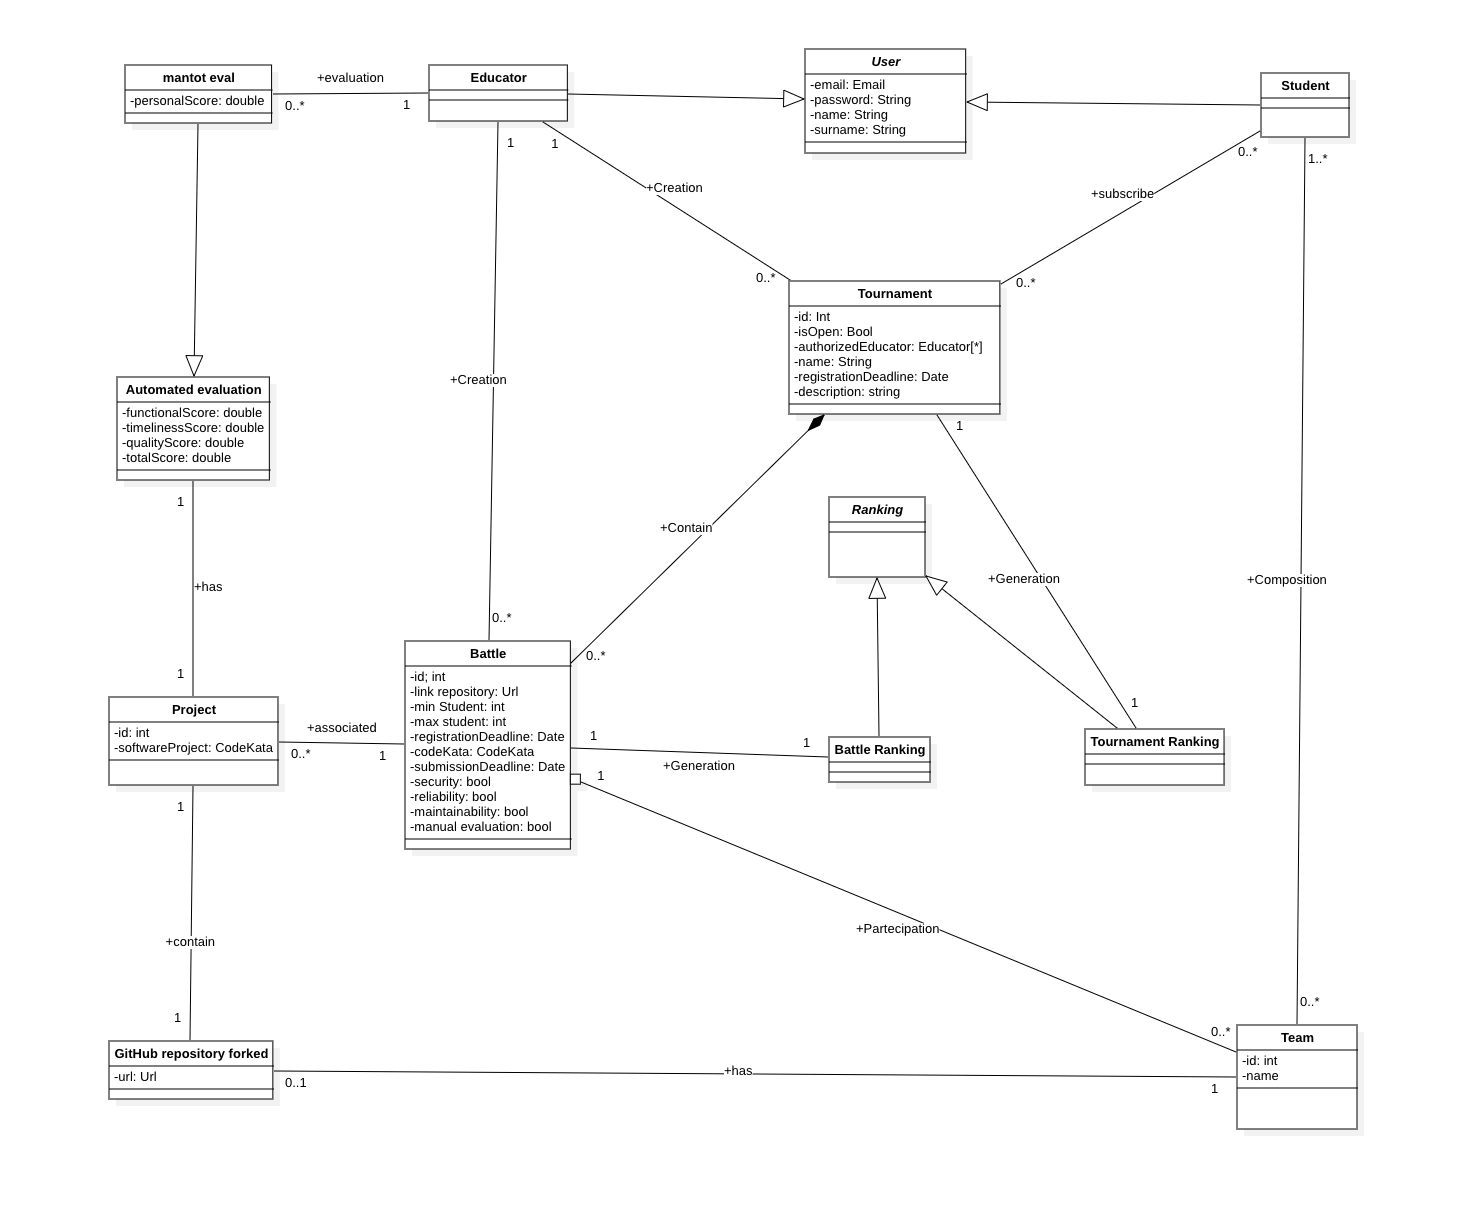
\includegraphics[width=0.95\textwidth]{ClassDiagram.png} % Sostituisci "nomefileimmagine" con il nome del tuo file immagine
  \caption{Descrizione dell'immagine} % Aggiungi una didascalia all'immagine
  \label{fig:etichetta} % Aggiungi un'etichetta per riferimenti futuri
\end{figure}




\subsection{StateChart Diagrams}
State diagrams describe the behaviour of the system while considering all possible states the objects can have when an event occurs.Di seguito sono riportati alcuni StateChart rappresentativi del sistema.
\\

\noindent\textbf{Login process}
    \begin{figure}[H]
  %\centering
  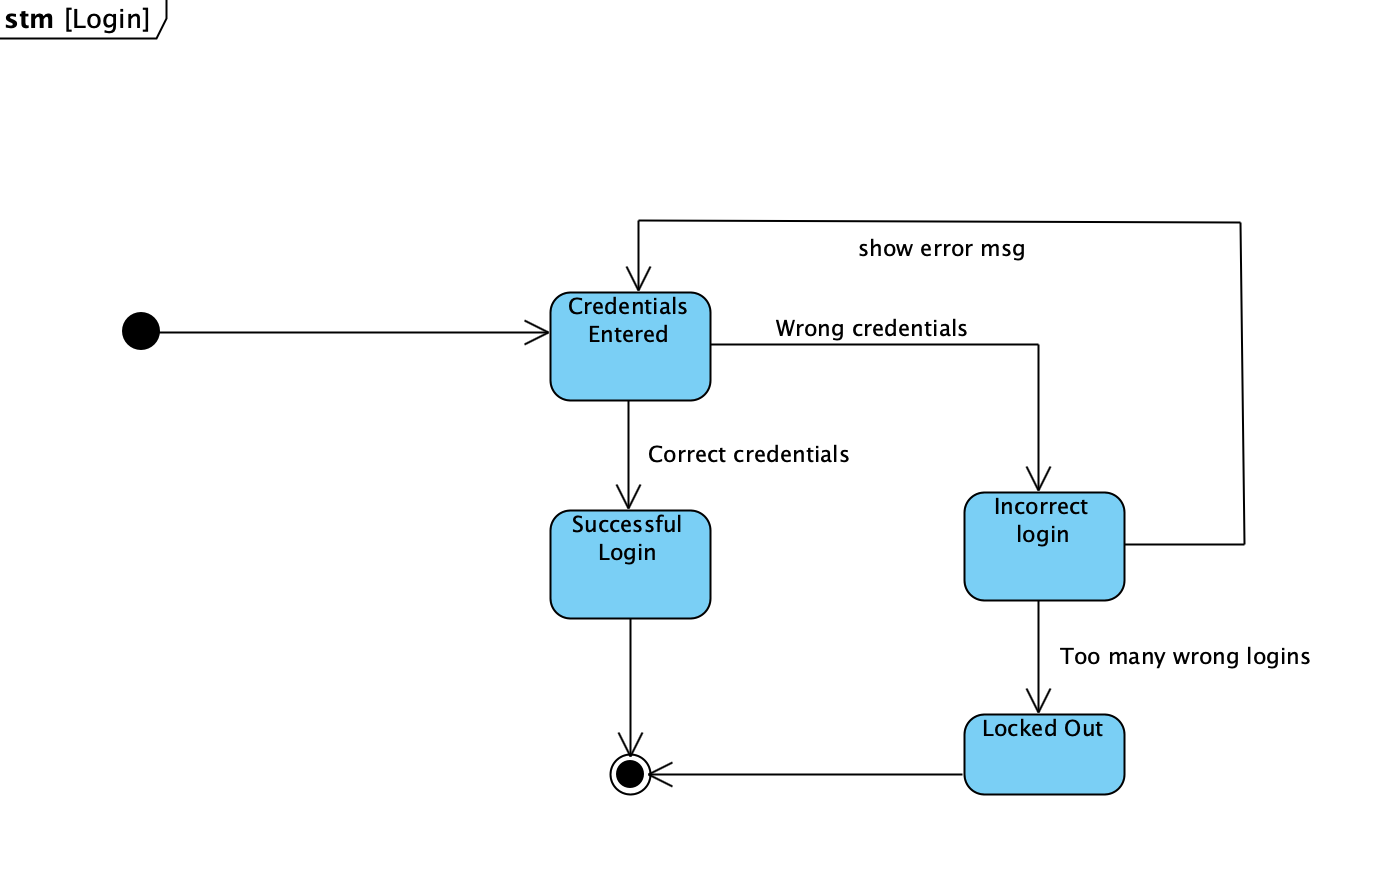
\includegraphics[width=1\linewidth]{StateChart/LoginStateChart.png} 
  \label{fig:immagine}
\end{figure}
\noindent Lo statechart visualizzato descrive il processo di autenticazione per un utente, sia esso un educatore o uno studente. Il diagramma inizia con lo stato "Credentials Entered" , che si ramifica in due percorsi possibili a seconda dell'esito della verifica delle credenziali.
Nel caso in cui le credenziali siano riconosciute come corrette, il processo prosegue nello stato "Successful Login" , concludendosi con successo e permettendo all'utente di accedere alle risorse protette. Al contrario, se le credenziali sono errate, il flusso di controllo viene indirizzato verso lo stato "Incorrect login" . Qui, all'utente viene presentato un messaggio di errore, indicando la necessità di riprovare l'inserimento dei dati. In caso di ripetuti fallimenti nell'autenticazione, indicati dal passaggio "Too many wrong logins" , il sistema trasferisce l'utente allo stato "Locked Out" , dove rimarrà fino a quando non verrà revocato il blocco dopo un determinato intervallo di tempo. 


\newpage
\noindent\textbf{Registration process}
    \begin{figure}[H]
  %\centering
  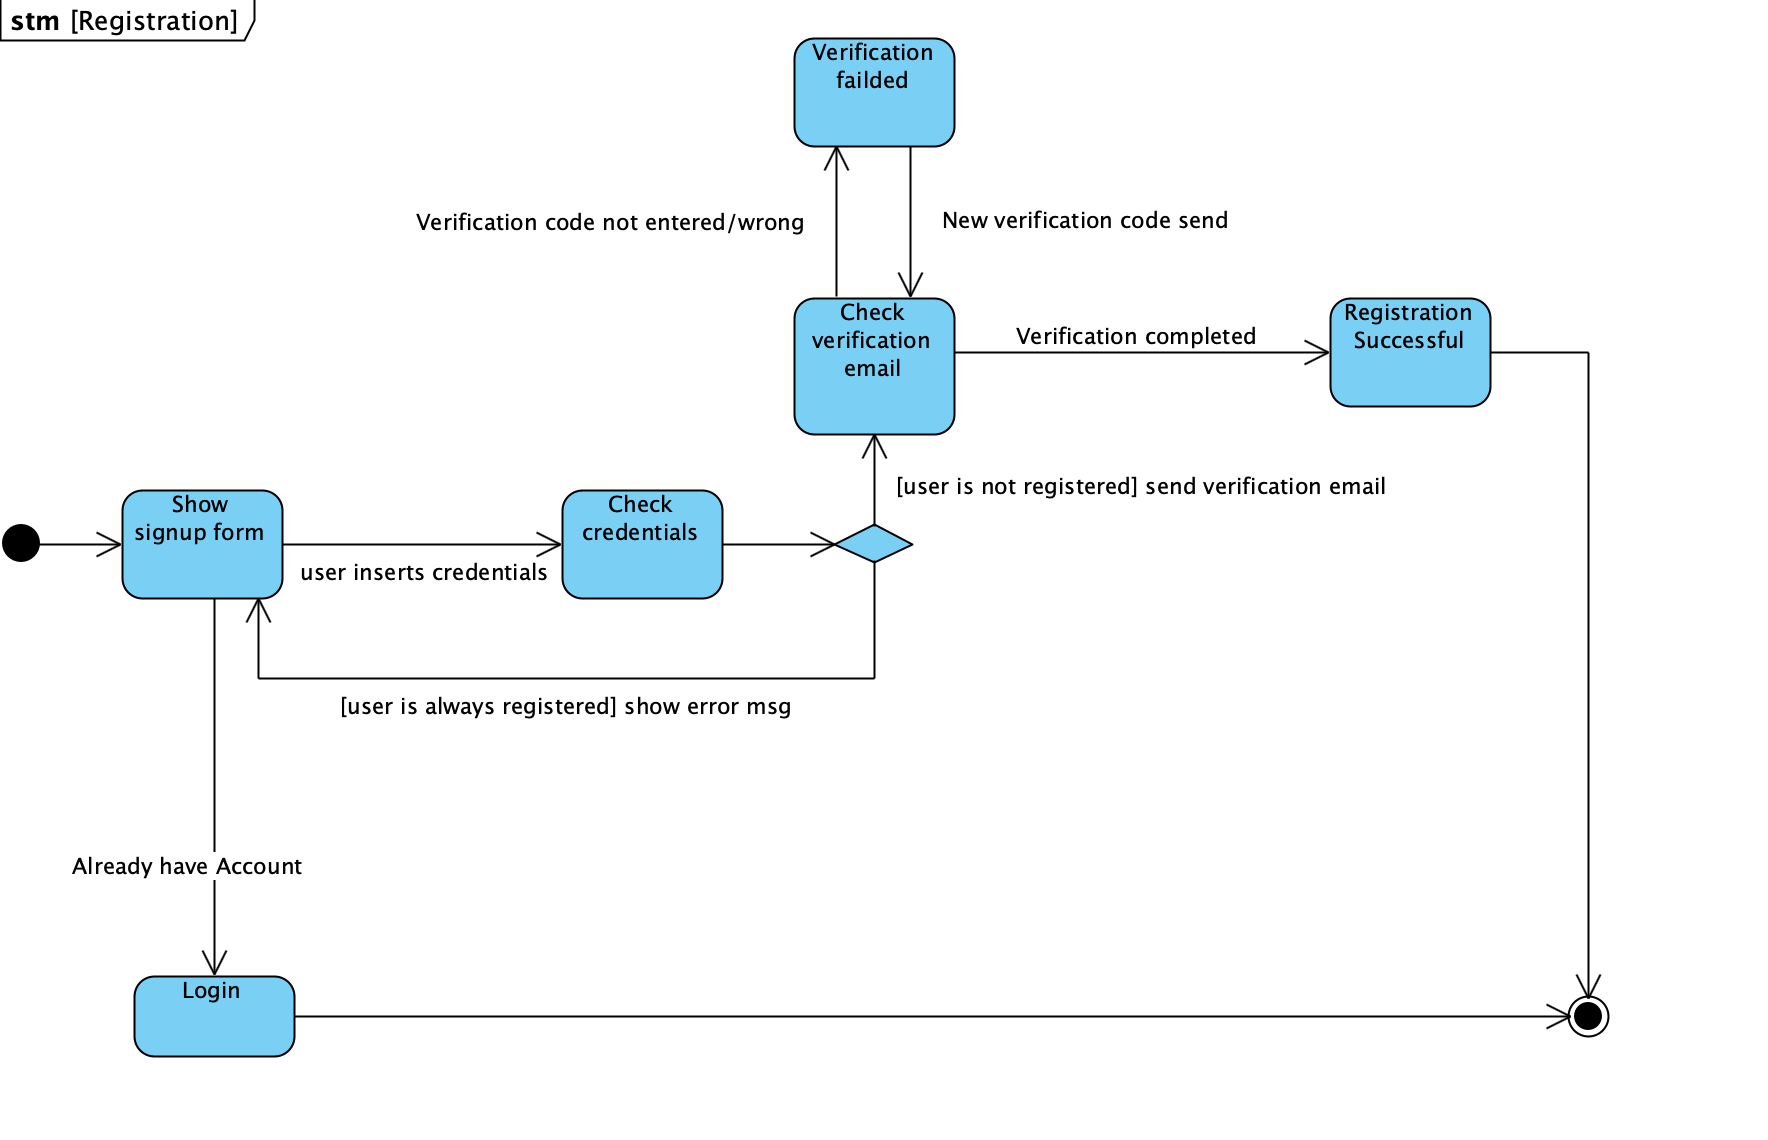
\includegraphics[width=1\linewidth]{StateChart/RegStateChart.png} 
  \label{fig:immagine}
\end{figure}
\noindent Questo statechart descrive il processo di registrazione per un utente,sia esso un educatore o uno studente.
Il primo stato "Show signup form"  rappresenta la visualizzazione del modulo di registrazione per l'utente.
Dopo che l'utente inserisce le credenziali, il processo prosegue con il controllo delle stesse nello stato "Check credentials" (Verifica credenziali). Se l'utente è già registrato, viene mostrato un messaggio di errore e l'utente viene reindirizzato al processo di login tramite lo stato "Login". Se l'utente non è registrato, il sistema procede con l'invio di una email di verifica, come indicato dal passaggio "Check verification email" (Verifica email di conferma). Se l'utente non inserisce il codice di verifica o inserisce un codice errato, si passa allo stato "Verification failed" (Verifica fallita), e viene inviato un nuovo codice di verifica.
Quando l'utente completa con successo la verifica inserendo il codice corretto, il processo di registrazione è completato con successo nello stato "Registration Successful" .
\\
\noindent\textbf{Evaluation process}
    \begin{figure}[H]
  %\centering
  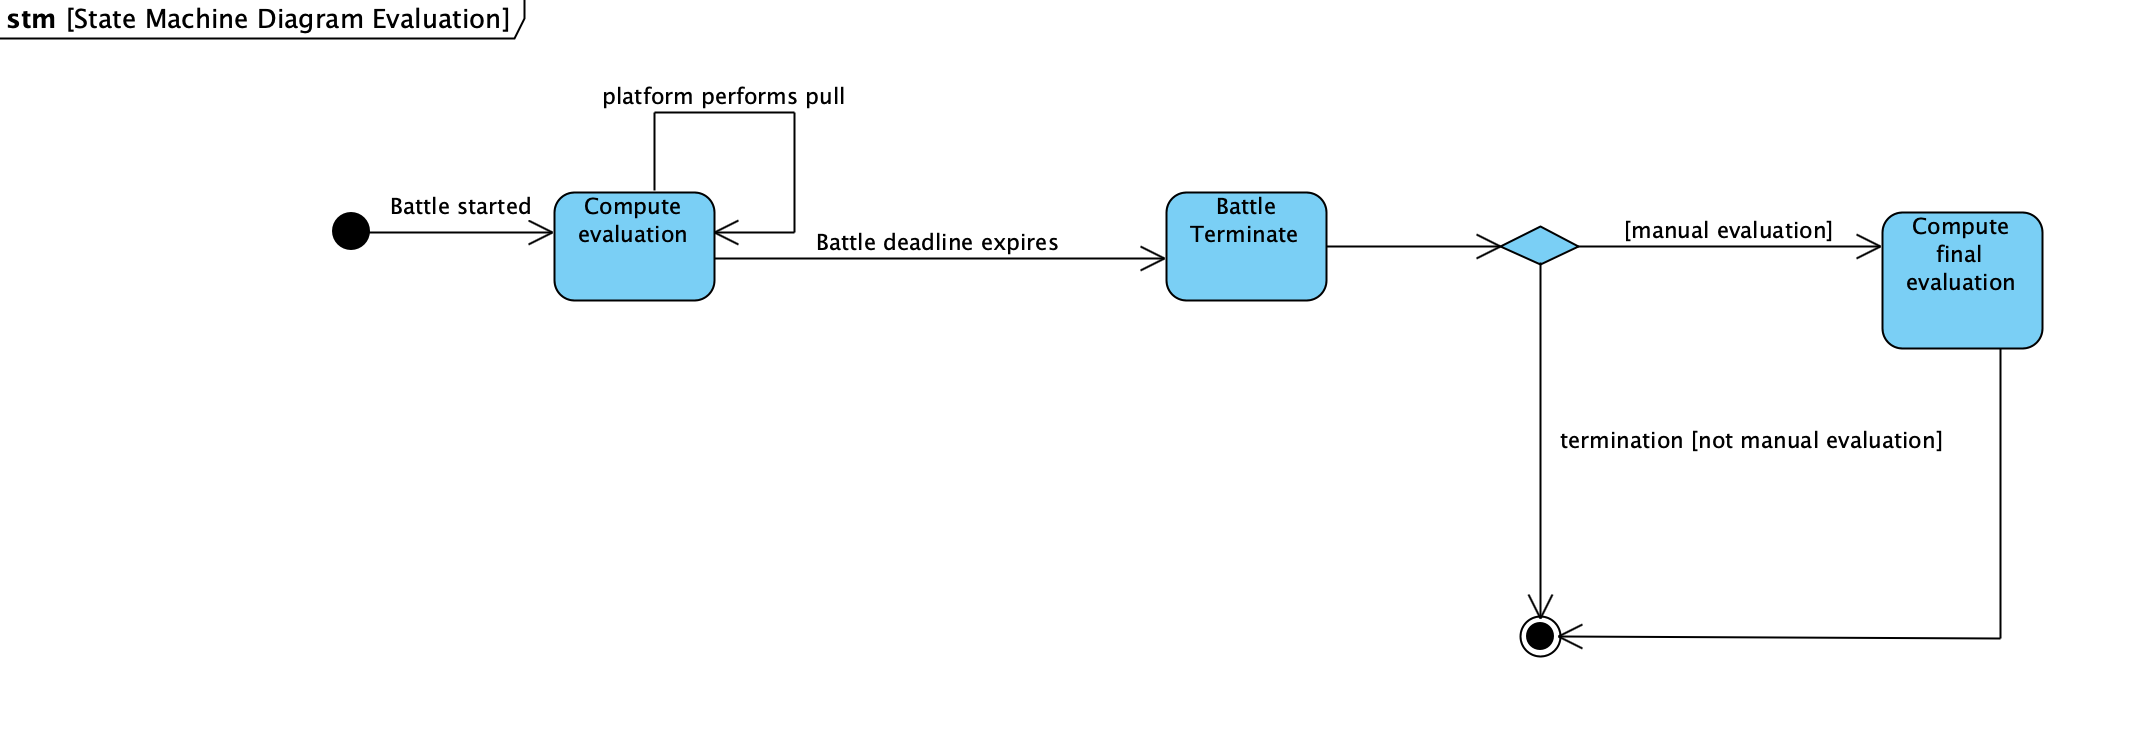
\includegraphics[width=1\linewidth]{StateChart/EvaluationStateChart.png} 
  \label{fig:immagine}
\end{figure}
\noindent Questo statechart rappresenta il processo di valutazione dei progetti in una battaglia. Nel primo stato, "Compute evaluation", viene eseguita automaticamente la valutazione del progetto di un team ogni volta che il sistema esegue un'operazione di pull per recuperare i dati necessari per la valutazione. Successivamente, il flusso si sposta allo stato "Battle terminated" se la "battaglia" è terminata, ovvero quando la scadenza per la presentazione della battaglia è raggiunta. A questo punto, se l'educatore ha impostato una valutazione manuale al momento della creazione della battaglia, il processo procede allo stato "Compute final evaluation", in cui l'educatore assegna un punteggio soggettivo a ciascun progetto. Successivamente, il processo si conclude. In caso contrario, il processo si conclude direttamente.\\

\noindent\textbf{Battle process}
    \begin{figure}[H]
  %\centering
  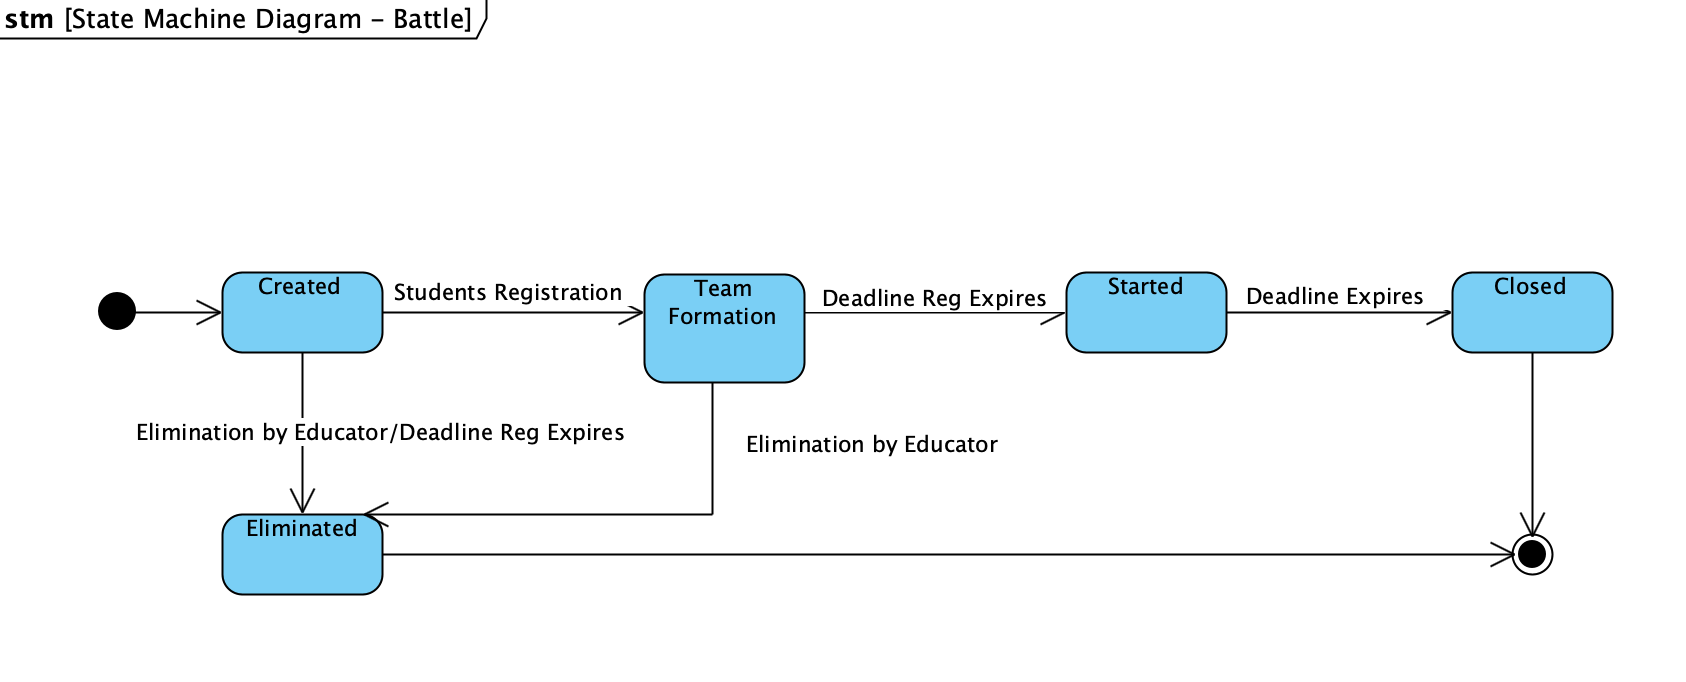
\includegraphics[width=1\linewidth]{StateChart/BattleStateChart.png} 
  \label{fig:immagine}
\end{figure}
\noindent Lo statechart mostrato in figura rappresenta il processo di evoluzione di una battaglia dalla sua creazione alla sua chiusura/eliminazione. Il processo inizia con lo stato "Creato", indicando che la battaglia è stata creata da un educator. Dopo la creazione dell'evento possono verificarsi tre situazioni:
 \begin{itemize}
     \item  Se nessuno studente prova a registrarsi per la battaglia e la registrazione deadline scade allora si va nello stato "Elimianted" e la battaglia viene automaticamente eliminata dal sistema.
     \item  Se nessuno studente si è ancora iscritto alla battaglia e l'educator creatore decide di eliminarla, si va nello stato "Elimianted" e la battaglia viene  eliminata dal sistema.
     \item  Se uno studente vuole registrarsi alla battaglia si passa allo stato "TeamFormation". In questo stato lo studente invita altri studenti per formare un team per la battaglia. Successivamente quando la deadline di registrazione scade si passa nello stato "Started" dove la battaglia è ufficialmente iniziata. Quando la deadline di submission scade la battaglia si chiude.

 \end{itemize}

\subsection{Product Functions}
This section provides  a summary of the major functions that the software will perform.\\

\begin{itemize}
    \item A general user can:
    \begin{itemize}
        \item Register
         \item Login
    \end{itemize}
\item A student can:
    \begin{itemize}
    \item Subscribe to a tournament
    \item Subscribe to a battle
    \item Form a team for the battle
    \item Explore the ranking of battles/tournaments
    \end{itemize}
\item  An educator can:
\begin{itemize}
    \item Create a tournament
    \item Create a battle
    \item Give permission to create battle within his tournament to other educators
    \item Manually evaluate student's projects.
\end{itemize}
\end{itemize}
\subsection{User characteristics}
As we have seen in the class diagram, there are two type of users: student and educator.
\subsubsection{Student}
A student is defined as someone eager to learn and enhance their programming skills. Students can navigate through dedicated pages on the CKB site to select the tournaments they are most interested in. They have the opportunity to participate in individual challenges or form teams, depending on the specific rules of each battle. In doing so, they compete with other students registered on the platform, testing their abilities and knowledge.
\subsubsection{Educator}
Anyone who wishes to create tournaments and battles, incorporating engaging and challenging tasks, is considered an educator. An educator has the freedom to upload various types of software projects within a battle, thus allowing anyone who registers to participate and compete. Moreover, educators have the ability to grant permissions to other educators to create battles within their tournaments. They also have the option to personally evaluate the tournament results or rely on the platform's default automated evaluation system.

\newpage
\subsection{Assumptions, dependencies and constraints}
\subsubsection{Assumptions}
These assumptions represent properties and/or conditions that the system takes for granted, primarily because they are beyond the control of the system itself. It is necessary to verify them to ensure the correct behavior of CKB.
\label{sec:assumptions_dependencies_and_constraints}%
\newcounter{da}
\setcounter{da}{0}
\newcommand{\cda}{\stepcounter{da}\theda}
\begin{center}
    \begin{longtable}{ |l|p{0.9\linewidth}| }
        \hline
        \textbf{ID} & \textbf{Description}                                                                                     \\
        \hline
        DA\cda      & Both educators and students must have an e-mail.                                         \\
         \hline
        DA\cda      & Students must have a  Github account.                                         \\
        \hline
        DA\cda      & Users who register on the CKB platform in the role of 'educator' are skilled  in designing meaningful and challenging code katas and also in evaluating them.                                                                           \\
        \hline
        DA\cda      & Users have consistent and reliable access to the internet and the necessary technology (computers, software development tools) to participate in coding battles and tournaments.                                                       \\
        \hline
        DA\cda      & The integration with GitHub and GitHub Actions functions correctly, allowing for seamless repository management, code submission, and automated workflow for the students’ projects.                                  \\
        \hline
        DA\cda      & Users who register on the CKB platform in the role of 'student'  have familiarity with programming languages,  GitHub, and test-driven development methodologies.        \\
        \hline
        \caption{Domain assumptions.}
        \label{tab:domainassmptn_tab}%
\end{longtable}
\end{center}


\subsubsection{Hardware Constraints}
The system has to run under the following worst-case conditions:
\begin{itemize}
    \item Internet Connection: Minimum 5 Mb/s.
    \item Screen Resolution: 1024x768.
    \item Modern Web like
\end{itemize}

\subsubsection{Regulatory policy}
The CKB application requires users to provide personal details, including their first name, last name, and email address. We assure users that their email addresses will not be utilized for any commercial or marketing purposes. All personal data collected will be handled and processed in strict adherence to the General Data Protection Regulation (GDPR), ensuring the highest standards of privacy.

